\documentclass[../../main.tex]{subfiles}

% 

\begin{document}
\chapter{Vlastnosti jader}

\subsection{Zadanie}

Struktura atomových jader, Hyperjádra, Antijádra, Elektrický náboj jádra, Poloměr jádra, Hmotnost jádra, Vazbová energie atomových jader, Energetické stavy atomových jader(energetické spektrum), Šířka energetické hladiny, Doba života stavu, Spin atomových jader, Parita stavu, Elektromagnetické momenty atomových jader, Magnetický dipolový moment, Elektrický kvadrupolový moment, Izotopický spin.

\section{Struktura atomového jádra}

Základní charakteristiky stabilních atomových jader: nukleonové číslo $A$, protonové číslo $Z$, neutronové číslo $N$, hmotnost $m$, elektrický náboj $q$, poloměr $r$, vazebná energie $E_v$, spin $S$, magnetický dipolóvý moment $\mu$ a elektrický kvadrupólový moment $Q_0$. Pro nestabilní atomová jádra jsou důležité ještě další charakteristiky jako je např. střední doba života, větvící poměr atd. Podle energetického stavu, ve kterém se jádra nacházejí je dělíme na ta v základním stavu a na ta ve stavu vzbuzeném. V ideálním případě by musela úplná informace o jádřě obsahovat strukturu a charakteristiky všech možných energetických stavů (hladin) jádra, způsoby a pravděpodobnosti pžřechodu jádra z jednoho stavu do druhého, pravděpodobnosti radioaktivního rozpadu jádra a charakteristiky emitovaných částic, účinné průřezy a charakter interakce jádra s jinými jádry, elementárními částicemi atd.

\subsection{Historie}

Původně si lidé mysleli, že atomové jádro je složeno z $A$ protonů a $A - Z$ elektronů (E. Rutherford $\Rightarrow$ lzetím vysvětlit celkový náboj a hmotnost). Tato domněnka byla ale vyvrácena, protože:

\begin{itemize}
	\item z relací neurčitosti ($\Delta p \Delta x \leq \hbar /2$) bychom očekávali energii elektronu v jádře přibližně $20 \mathrm{MeV}$ $\rightarrow$ ve skutečnosti se energie elektronu pohybuje řádově v rozmezí $0,02 - 13 \mathrm{MeV}$,
	\item Coulombická interakce by nebyla schopna udržet elektron v jádře,
	\item spin deuteronu je roven $1$, ale pokud by se skládal ze dvou protonů a jednoho elektronu, pak by jeho spin byl poločíselný,
	\item jádra s lichým počtem elektronů by měly velké mag. momenty $\Rightarrow$ např. deuteron by měl mag. moment podobný elektronu.
\end{itemize}

\section{Základní definice}

Strukturu atomového jádra vystihují tři čísla:

\begin{itemize}
	\item PROTONOVÉ ČÍSLO $Z$ (někdy také atomové číslo) $=$ udává počet elektronů v obalu neutrálního atomu, počet protonů v jádře atomu příslušného prvku a také pořadové číslo prvku v periodické soustavě,
	\item NEUTRONOVÉ ČÍSLO $N$ $=$ udává počet neutronů v atomovém jádře,
	\item NUKLEONOVÉ ČÍSLO $A$ $=$ udává počet nukleonů (protonů $+$ neutronů) v jádře.
\end{itemize}

Pro tato tři čísla platí vztah

\begin{equation}
A = Z + N.
\end{equation}

Prvky pak značíme následujícím způsobem

\begin{equation}
^{A}_{Z}X_N.
\end{equation}

Nejdůležitějším číslem je NUKLEONOVÉ ČÍSLO $A$, které slouží k rozlišení jednotlivých izotopů.

\begin{itemize}
	\item IZOTOPY: $Z_1 = Z_2, N_1 \neq N_2, A_1 \neq A_2$,
	\item IZOTONY: $Z_1 \neq Z_2, N_1 = N_2, A_1 \neq A_2$,
	\item IZOBARY: $Z_1 \neq Z_2, N_1 \neq N_2, A_1 = A_2$,
	\item IZOMERY: $Z_1 = Z_2, N_1 = N_2, A_1 = A_2$, ale liší se energetickým stavem, doba života je díky potlačení pravděpodobnosti přechodu mezi hladinami se značně rozdílným impulsmomentem nadstandardně velká (až několik hodin) 
	\item NUKLIDY: atomy mající stejný počet protonů a neutronů
	\item RADIONUKLIDY: nuklidy složené z atomů se stejným energetickým stavem, které podléhají samovolnému štěpení
	\item ZRCADLOVÁ JÁDRA: $Z_1 = N_2$ a $Z_2 = N_1$
\end{itemize}

Protonová a neutronová čísla $Z$ a $N$ mají značný význam pro stavbu atomových jader. Podle sudosti, resp. lichosti $Z$, resp. $N$ lze stabilní nuklidy rozdělit do čtyř skupin, které jsou uvedené v tabulce \ref{sf6tab:1}. Nejvíce stabilních nuklidů tvoří jádra sudo-sudá. Licho-liché stabilní nuklidy jsou pouze čtyři: $^{2}_{1}H$, $^{6}_{3}Li$, $^{10}_{5}B$, $^{14}_{7}N$.

\begin{itemize}
	\item SUDO-SUDÁ JÁDRA: N/Z = 4, 12, 16, 20, 24 $\rightarrow$ maxima  vazbové energie na nukleon
\end{itemize}

 \begin{table}[h!]
 	\centering
 	\begin{tabular}{|c||c|c|}
 		\hline $Z$ & $N$ & Počet stabilních nuklidů  \\ 
 		\hline \hline sudé  & sudé & 165 \\ 
 		\hline \hline sudé & liché & 55  \\
 		\hline \hline liché  & sudé & 50 \\ 
 		\hline \hline liché & liché & 4  \\
 		\hline 
 	\end{tabular} 
 	\caption{Rozdělení stabilních nuklidů podle sudosti a lichosti protonového a neutronového čísla.}
 	\label{sf6tab:1}
 \end{table}

\section{Hyperjádra}

\begin{itemize}
	\item hyperon $\Lambda = uds$
	\item hyperon $\Lambda_c = udc$ 
\end{itemize}

HYPERJÁDRA jsou atomová jádra, která obsahují kromě nukleonů nejméně jeden hyperon a mají tedy nenulovou podivnost. Termínem hyperon označujeme ve fyzice elementárních částic baryon (tj. hadron složený ze tří kvarků) mající nenulovou podivnost a interagující silnou interakcí. Význam hyperjader spočívá v tom, že lze jejich prostřednictvím studovat atomová jádra (zvláště stavy ležící pod Fermiho hladinou - $ \Lambda $ se může usadit i na slupkách, na kterých to nukleonům znemožňuje Pauliho vylučovací princip) a také $ \Lambda - \Lambda $ a $\Lambda - N$ interakce. Nejsnadněji se studují hyperjádra obsahující $\Lambda _0$, která žijí dostatečně dlouho (v porovnání s jaderným časem žijí hyperjádra poměrně dlouho, neboť $\tau _ \Lambda = 2,6.10^{-10} \mathrm{s}$). Byla také připravena hyperjádra obsahující hyperon $ \Sigma ^0 $ i hyperjádra s vícenásobnou podivností. V současné době je známo více než třicet hyperjader. Poprvé bylo hyperjádro pozorováno v roce 1952. V roce 2010 bylo připraveno první antihyperjádro. 

Hyperjádra označujeme spodním levým indexem $ \Lambda $ (případně $ \Sigma ^0 $) - např. $^{56}_{\Lambda}Fe$, hyperjádra s vícenásobnou podivností $^{6}_{\Lambda \Lambda}He$, antihyperjádro $^{3}_{\overline{ \Lambda }}\overline{He}$.

Hyperjádra mohou vznikat několika způsoby:
\begin{itemize}
	\item změnou podivnosti jádra např. při prostém zachycení hyperonu nebo při zachycení hyperonu či podivného mezonu a jeho interakci s jaderným nukleonem
	\item rozpadem jiného hyperjádra
	\item zisk prostřednictvím vesmírného záření
	\item záchyt kaonu 
	\begin{equation}
	^{14} C (K^-, \pi ^-)  ^{14}_{\Lambda}C,
	\end{equation}
	\begin{equation}
     ^{12} C (K^-, \pi ^+)  ^{12}_{\Sigma ^-}Be.
	\end{equation}
\end{itemize}

Hyperjádra jsou velmi nestabilní objekty. Jejich střední doba života leží většinou v intervalu mezi $10^{-11} - 10^{-10} \mathrm{s}$. Rozpadají se baryonovým rozpadem (výsledkem je baryon) slabou interakcí buď mezonovým nebo bezmezonovým rozpadem. Mezonový rozpad probíhá rozpadem hyperonu v jádře za vzniku $\pi ^-$ nebo $\pi ^0$ 


\begin{equation}
\Lambda \rightarrow p + \pi ^-   ~~~~~~~ ...63,9 \%,
\end{equation}
\begin{equation}
\Lambda \rightarrow n + \pi ^0   ~~~~~~~ ...35,8 \%.
\end{equation}

U lehčích jader může dojít i k současnému uvolnění nukleonu nebo rozštěpení jádra (přičemž zbylé jádro má velkou vazebnou energii na nukleon). Při bezmezonovém rozpadu dochází k interakci hyperonu s protonem ($\Lambda + p \rightarrow p + n$) nebo neutronem ($\Lambda + n \rightarrow n + n$) a pozoruje se zpravidla u těžkých jader. 

Vazbové energie hyperjader se pohybují v rozmezí $0,06 \mathrm{MeV} \leq E_v \leq 20 - 30 \mathrm{MeV}$.

\subsection{Exotická jádra}

Super těžká jádra, která jsou vzdálená od linie stability:
\begin{itemize}
	\item $\rightarrow$ s velkým přebytkem neutronů
	\item $\rightarrow$ s velkým deficitem neutronů (přebytkem protonů)
\end{itemize}
Pro vysoká $A$ a $Z$ stabilita klesá - existence magických čísel $\rightarrow$ ostrov stability. Prokázána jádra po $Z = 112$.

\subsection{Dvojitě magická jádra}
\begin{itemize}
	\item MAGICKÁ ČÍSLA = 2, 8, 20, 28, 50, 82, 126 $\rightarrow$ pozorované hodnoty $N$ a $Z$ se zvýšenou stabilitou
\end{itemize}

$^{100} Sn$ je takové jádro s největším počtem neutronů a protonů.

\subsection{Vysoce vzbuzené stavy}
\begin{itemize}
	\item $\rightarrow$ s velmi vysokou energií
	\item $\rightarrow$ s velmi vysokým spinem
	\item $\rightarrow$ s velkými deformacemi - kvadrupólovými momenty
\end{itemize}

\section{Antijádra}

Po objevu antiprotonu $\overline{p}$ (r. 1955) a antineutronu $\overline{n}$ (r. 1956) se stala aktuální otázkou existence antijader a antiatomů (obal antiatomů obsahuje pozitrony). V r. 1965 bylo poprvé experimentálně dokázáno, že z antičástic mohou být sestaveny komplexy stejného typu jako z částic. Skupina amerických fyziků pod vedením L. Ledermana získala na urychlovači a zaregistrovala první antijádro - antideuteron $\overline{d}$ (tj. vázaný stav $\overline{p}$ a $\overline{n}$). V roce 1969 v experimentech na urychlovači protonů bylo skupinou fyziků zaregistrováno antijádro $^{3} \overline{He}$ a o pět let později bylo objeveno antijádro tritia $^{3} \overline{H}$ V roce 1999 byl připraven antivodík $^{1} \overline{H}$.

Studium interakce antineutronu s neutronem ukázalo, že může vznikat vázaný stav s vazbovou energií menší, než je celková energie páru antinukleon-nukleon. V experimentu se tyto vázané stavy mohou projevovat ve tvaru bosonových rezonancí s malým spinem a hmotností blízkou dvojnásobku hmotnosti nukleonu. Podobné rezonance byly zjištěny experimentálně.

\section{Poloměr jader}

Jádro je kvantový objekt, tudíž není zcela správné hovořit o jeho poloměru (podobná situace je i v atomové fyzice, kde hranice atomu také není přesně daná, protože vlnové funkce vnějších elektronů monotónně klesají). Naše představa o něm je pouze aproximativní, různé představy dávají různé výsledky. Výsledky experimentů lze shrnout formulí pro poloměr atomového jádra
\begin{equation}
R = r_0 A ^{1/3},
\end{equation}
kde $A$ je nukleonové číslo a $r_0$ nabývá hodnoty z intervalu $\langle1,05; 1,45\rangle ~\mathrm{fm}$, nejčastěji používaná je hodnota $1,3 ~\mathrm{fm}$.

Předpokládáme-li, že jádro je koule, můžeme spočítat objem připadající na jeden nukleon: $V_0 = V/A = konst.$. Z tohoto výsledku vyplývá, že jaderné síly jsou NASYCENÉ. Číselná hodnota hustoty jádra, která nabývá velmi vysoké hodnoty $\rho _{AJ} = 10^{14} g.cm^{-3}$.

\subsection{Měření poloměru jader}

\begin{itemize}
	\item hustota jádra: $\rho (x) = | \psi (x) |^2$
\end{itemize}
Rozměry jádra jsou charakterizovány rozdělením hmoty a náboje:
\begin{itemize}
	\item střední kvadratický poloměr: $R^{2}_{rms} = <r^2> = \dfrac{\int r^2 \rho (r) dV}{\int \rho (r) dV}$
	\item poloměr ekvivalentního homogenního rozdělení: $R = \sqrt{\dfrac{5}{3}} R_{rms}$
	\item místo, kde hustota spadne na polovinu: $\rho (r) = \dfrac{\rho (0)}{2}$
	\item tloušťka povrchové vrstvy, kde $\rho (r)$ klesne z $90 \%$ na $10 \%$
\end{itemize}

Základní metody měření:
\begin{itemize}
	\item citvivé na rozdělení el. náboje
	\begin{itemize}
	    \item ROZPTYL RYCHLÝCH ELEKTRONŮ - elektron = neinteraguje silně $\Rightarrow$ rozdělení el. náboje. Rozlišovací schopnost částice závisí na de Broglieho vlnové délce $\lambda = \dfrac{h}{p}$. Pro rozměry jádra $\sim$ 10 $\mathrm{fm}$ potřebujeme $\lambda \leq 10 \mathrm{fm}$ $\Rightarrow$ $p \geq 100 ~\mathrm{MeV}$. Při menší vlnové délce vidíme větší detaily. 
	    
	    Analogie s optikou: 
	    \begin{itemize}
	    	\item jádro - 2D pevný terčík o průměru $D = 2R$
	    	\item pro $ \lambda \sim D$ nastává difrakce
	    	\item první minimum $\Theta = \sin^{-1} (1,22 \dfrac{\lambda}{D})$
	    \end{itemize} 
	    
	    Elektron při $p \sim 100 ~\mathrm{MeV}$ je relativistická částice se spinem 1/2 a mag. momentem.
	    
	    Rozptyl na bodovém náboji: 
	    \begin{equation}
	    \left( \dfrac{d \sigma}{d \Omega }\right)_{Ruth} \rightarrow  \left( \dfrac{d \sigma}{d \Omega }\right)_{Mott} = \left(  \dfrac{Z_1 Z_2 e^2}{8 \pi \epsilon_0 |p| c \beta}\right)^2 \dfrac{1 - \beta^2 \sin^2 (\Theta/2)}{\sin ^4 (\Theta /2)}. 
	    \end{equation}
	    Rozptyl na terči s hustotou náboje $\rho (r)$:
	    
	    	\begin{center}
	    		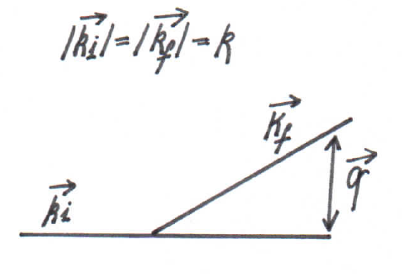
\includegraphics[width=0.4\textwidth]{rych_el.png}		
	    	\end{center}
	    
	    \begin{equation}
	    \left( \dfrac{d \sigma}{d \Omega}\right) _{exp}  = \left(\dfrac{ d \sigma }{d \Omega}\right)_{Mott} \left| F (q^2)\right|,  
	    \end{equation}
	    kde $F(q)$ je formfaktor $\rightarrow$ struktura terčíku.
	    \begin{equation}
	    F(q^2) = \int \rho (\vec{r}) \exp ( i \vec{q}\cdot \vec{r}) d^3 \vec{r}, ~~~~~~~~~ \vec{q} = \vec{k_i} - \vec{k_f}.
	    \end{equation}
	    
	    Pro elestický rozptyl je $q = 2k \sin (\Theta /2)$, pro rozptyl na bodovém náboji: $q^2 \rightarrow 0$ $\rightarrow$ $F(q^2) \rightarrow 1.$
	    
	    Teoreticky lze získat rozdělení náboje: $\rho (r) = \dfrac{1}{(2 \pi)^3} \int d^3 q F(q^2) \exp \left(-\dfrac{i}{\hbar} \vec{q}\cdot \vec{r}\right).$
	    
	    Rozdělení hmoty v jádře $\rightarrow$ rozdělení náboje získáme zpětnou Fourierovou transformací.
	    
	    Závěry: $\rightarrow$ centrální část s konstantní hustotou ($\pm 1 \%$) a povrchová oblast o tloušťce $\sim$ $2,4 ~\mathrm{fm}$.
	    
	    ~~~~~~~~~~$\rightarrow$ poloměr je dobře popsán jako $R = R_0 A^{1/3}$.
	    
	    \item IZOTOPOVÝ POSUN - jádro má konečný rozměr - modifikace el. potenciálu uvnitř: 
	    \begin{equation}
	    V'(r) = - \dfrac{Z e^2}{2 \pi \epsilon_0 R} \left( \dfrac{3}{2} - \dfrac{1}{2} \dfrac{r^2}{R^2}\right) ~~~~~~~~~~~~ r<R
	    \end{equation}
	    $\Rightarrow$ rozdělení potenciálu uvnitř homogenní koule
	    
	    Lineární závislost souhlasí se závislostí poloměru $\sim A^{1/3}$. Rozdíl mezi sudými a lichými jádry. Z izotopového odstupu spektrálních čar - změna čáry souvisí s tím, o jaký izotop se jedná a jetli vlnové funkce byly počítány s intenzitou pro bodový náboj, tj. $I \sim \dfrac{1}{r}$, anebo jestli byly počítány s intenzitou danou pro nabitou kouli, pro kterou je $I \sim r$ pro $r \in < 0,R>$ a $I \sim \dfrac{1}{r}$ pro $ r \in <R, \infty>$.
	    
	    	\begin{center}
	    		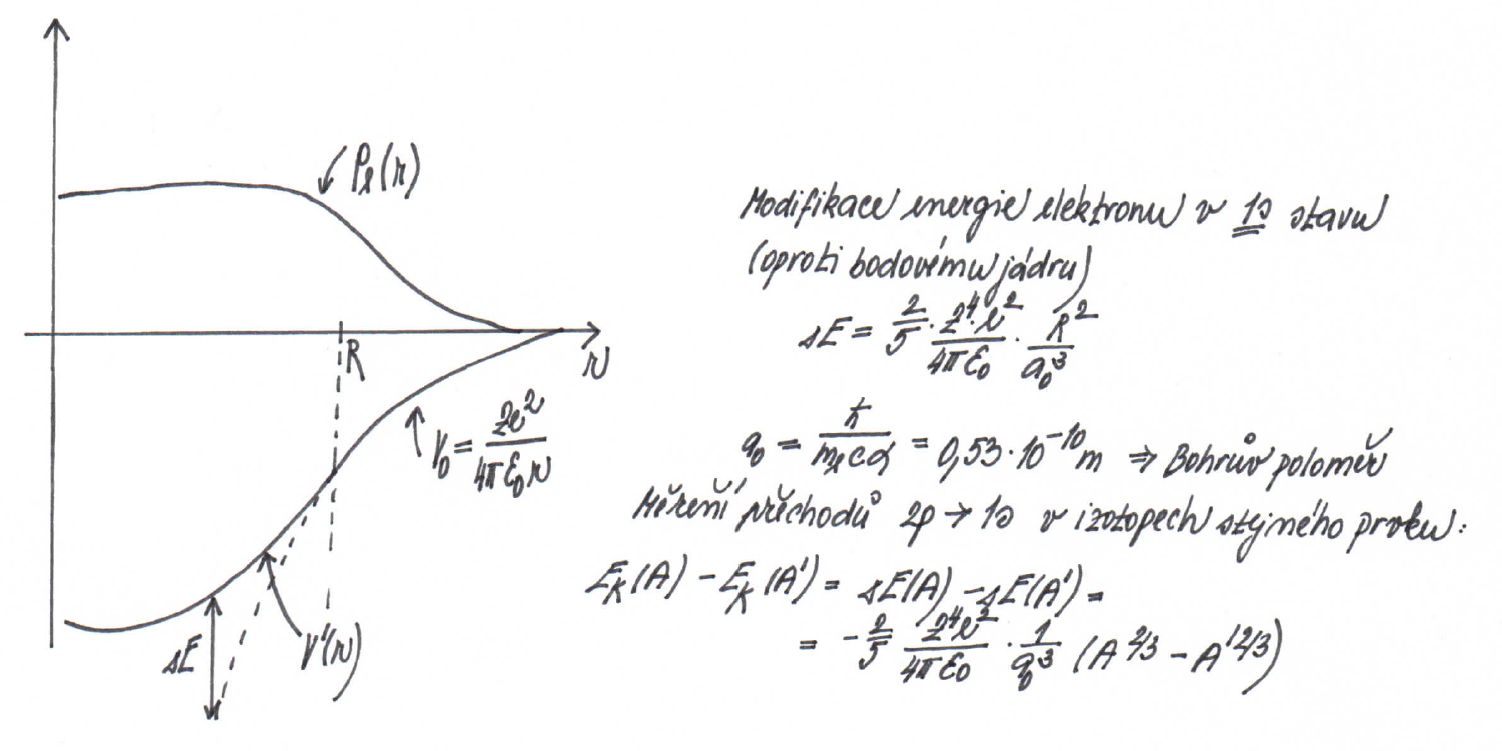
\includegraphics[width=1\textwidth]{izot_posun.png}		
	    	\end{center}
	    
	    \item Z RENTGENOVÝCH SPEKTER MIONOVÝCH ATOMŮ - izotopový posun lze vylepšit použitím mionů: $\dfrac{m_ {\mu}}{m_e} = 207 $ $\Rightarrow$ miony jsou vázány mnohem blíže u jádra. Mion se zachytí v atomovém obalu a rychle (během $10^{-14} ~\mathrm{s}$ až $10š{-13} ~\mathrm{s}$) se dostane na K slupku, která vzhledem k hmotnosti mionu zasahuje do jádra. Hodnoty energie tak budou citlivé na velikost jádra. Rentgenová emise funguje analogicky jako u elektronů, proměřením spektra lze tedy získat závěry o poloměru atomových jader. Nejpřesněji se touto metodou určují hodnoty poloměru pro těžká jádra.
	    
	    \item Z ROZDÍLU VAZEBNÝCH ENERGIÍ ZRCADLOVÝCH JADER - zrcadlová jádra lze získávat pomocí $\beta$-rozpadu, jehož energie je rovna
	    \begin{equation}
	    	\begin{aligned}
	    	E_{rozp} & = E_{\beta _{max}}= (m(A,Z) - m(A, Z-1) - m_e)c^2 =  [ (A-Z)m_n + Z m_p - \\
	    	&- \dfrac{W(A,Z)}{c^2} - \left( (A-Z+1)m_n + (Z-1)m_p - \dfrac{W(A,Z-1)}{c^2} - m_e\right) ] c^2 \\  
	    	& = W(A,Z-1) - W(A,Z) - (m_n - m_p + m_e)c^2 = W(A,Z-1) - W(A,Z) - 1,8 ~\mathrm{MeV},	
	    	\end{aligned}
	    \end{equation}	
	    a navíc ještě platí vztah pro elektrostatickou energii objektu o hustotě energie $\rho (r)$
	    \begin{equation}
	    E_c = \dfrac{1}{8 \pi \epsilon _0} \int \dfrac{\rho (r_1) \rho (r_2)}{|\vec{r_1} - \vec{r_2}|} dV_1 dV_2
	    \end{equation}	
	    a pro Coulombickou energii
	    \begin{equation}
	    W_c = - \dfrac{1}{4 \pi \epsilon _0} \dfrac{3}{5} \dfrac{Z^2 e^2}{R}
	    \end{equation}
	    a tedy dále 
	    \begin{equation}
	    \begin{aligned}
	    E_{rozp} = E_{\beta _{max}} & = W(A, Z-1) - W(A,Z) - 1,8~\mathrm{MeV} \\
	    & = \dfrac{3}{5} \dfrac{e^2}{R} (Z^2 - (Z-1)^2) - 1,8~\mathrm{MeV} \\
	    & = \dfrac{3}{5} \dfrac{e^2}{R} (2Z-1) - 1,8~\mathrm{MeV}
	    \end{aligned}
	    \end{equation}
	    \begin{equation}
	    \Rightarrow r_0 = (1,28 \pm 0,05)~\mathrm{fm}.
	    \end{equation}	
	
	\end{itemize}
	\item citlivé na rozdělení (silně interagující) hmoty
	\begin{itemize}
		\item RUTHERFORDŮV ROZPTYL - ukázka rozdělení: homogenní rozdělení (koule): 
		\begin{equation}
		\rho (r) = \rho _0 ~~~~~~ r < R,
		\end{equation}
		\begin{equation}
		\rho (r) = 0 ~~~~~~ r > R.
		\end{equation}
		\begin{equation}
		R_{rms} = \left\langle r^2 \right\rangle ^{1/2} = \dfrac{3}{5} R.
		\end{equation}
		
		WOOD-SAXON (Fermi) $\rightarrow$ popisuje jedarný potenciál: 
		\begin{equation}
		\rho (r) = \dfrac{\rho _0}{1 + \exp \left[ \dfrac{r - R}{a}\right] },
		\end{equation} 
		\begin{equation}
		R_{rms} = \left\langle r^2 \right\rangle ^{1/2} = \sqrt{\dfrac{3}{5} \left( R^2 + \dfrac{7}{3} \pi^2 a^2 \right)},
		\end{equation}
		kde $\rho _0 = 0,08$ neutronů či protonů na $\mathrm{fm^3}$, $R = 1,2.A^{1/3}$ ... hustota klesne na 1/2, $a = 0,6 ~\mathrm{fm}$ ... reguluje, jak rychle vrstva klesá.
		
		Klasický přístup, v CMS: 
		\begin{equation}
		\dfrac{d \sigma}{d \Omega} = \left( \dfrac{Z_1 Z_2 e^2}{16 \pi \epsilon _0 E} \right) ^2 \dfrac{1}{\sin ^4 \left( \dfrac{\Theta}{2}\right) }.
		\end{equation}
		Maximální přiblížení $\alpha$-částice: 
		\begin{equation}
		r_{min} = \dfrac{b \cos (\Theta /2)}{1 - \sin(\Theta/2)}.
		\end{equation}
		Při $\Theta = \pi$: $r_{min} = \dfrac{2 Z e^2}{4 \pi \epsilon _0 E}$.
		
			\begin{center}
				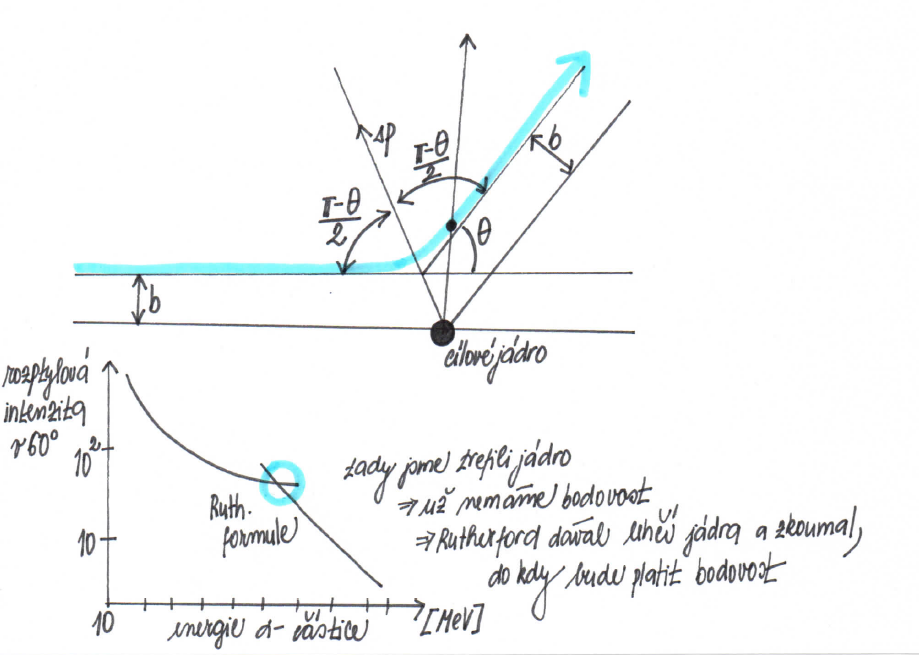
\includegraphics[width=1\textwidth]{ruth.png}		
			\end{center}
			
		\begin{itemize}
			\item Rutherfordův rozptyl $\alpha$-částice
			
			Experimentální výsledky:
			\begin{equation}
			R = r_0 A^{1/3},
			\end{equation}
			\begin{equation}
			r_0 = (1,52 \pm 0,08).10^{-15} ~\mathrm{m},
			\end{equation}
			kde $R$ je vzdálenost, kde začnou působit jaderné síly.
			
			Vliv silné interakce rychle klesá při $r>R$ $\rightarrow$ krátký dosah.
		
		\end{itemize}
		\item ROZPTYL RYCHLÝCH NEUTRONŮ $\rightarrow$ špatně se detekují + špatně se mění $E$, citlivé k rozdělení hmoty, složený objekt, nelze urychlovat, použití sekundárních svazků - horší energetické rozlišení, těžší detekce - horší rozlišení, možnost absorbce v jádře - použití komplexního potenciálu, klasicky $\sigma = \pi R^2$, v QM až $\sigma = 2 \pi R^2$ (absorbce + pružný rozptyl), nejpřímější způsob měření rozdělení silných nábojů. Změřená velikost: $1,3 - 1,4~\mathrm{fm}$. Širší povrchová vrstva: $3,2 ~\mathrm{fm}$.
		
		\item Z $\alpha$-ROZPADŮ TĚŽKÝCH JADER - potenciál, jenž cítí $\alpha$-částice, lze aproximovat potenciálovou jámou. $A$ je oblast silné interakce, $B$ je oblast klasické Coulombické interakce. $\alpha$ částice se pohybuje v potenciálové jámě, ale z kvantového hlediska je možnost, že nastane tunelový jev. V detektoru pak lze detekovat kinetickou energii $T_{kin}$ $\alpha$-částice. Pravděpodobnost protunelování je dána obsahem plochy $C$. 
		
		\begin{center}
			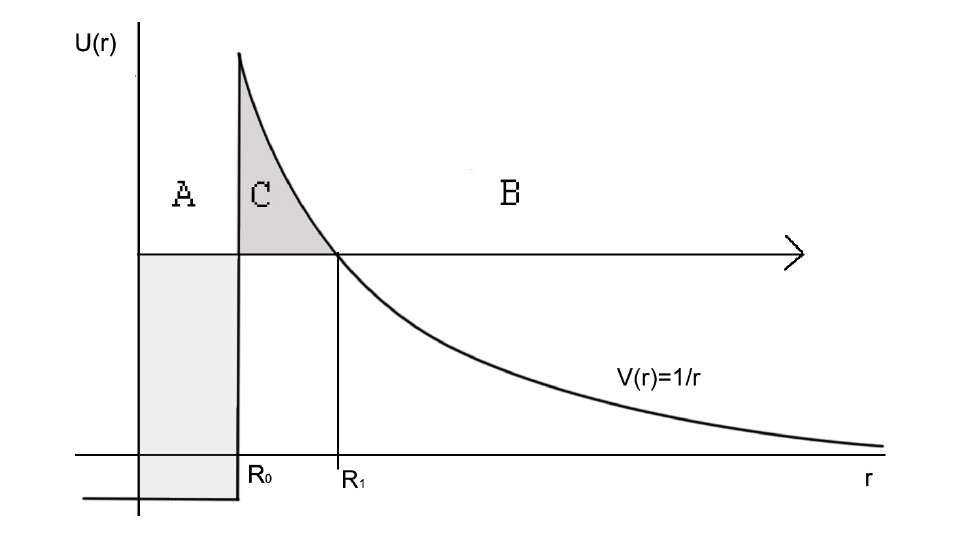
\includegraphics[width=0.8\textwidth]{tunelovani.png}
			\captionof{figure}{Pravděpodobnost protunelování $\alpha$-částice Coulombickou bariérou}		
		\end{center}
		
		\item $\pi$-ATOMY - obdobné jako $\mu$-atomy s tím rozdílem, že piony interagují silně. Poté co se dostanou blízko jádru (s1-orbit, budou interagovat s nukleony a budou absorbovány v jádře). Pion je el. nabitý (stejně těžký jako mion) $\rightarrow$ interaguje silně $\rightarrow$ interakce s jádrem.
	\end{itemize}
\end{itemize}


\section{Náboj atomových jader, rozložení náboje a hmoty v jádře}

Náboj atomového jádra udáváme jako $q = Z e$, kde $Z$ je počet protonů v jádře a $e = 1,602.10^{-19} ~\mathrm{C}$ je velikost elementárního náboje. Rozložení elektrického náboje v jádře je určeno především uspořádáním protonů. Na rozložení hmoty mají vliv jak protony, tak i neutrony. 

Rozložení hmoty a náboje v jádře může být studováno analyzováním srážek různých částic s jádrem. Rozložení náboje lze nejsnáze vyšetřovat pomocí částice, která interaguje jenom s nábojem jádra - v tomto ohledu je ideální částicí elektron (elektromagnetická interakce je velmi dobře popsána, tudíž pružná srážka elektronu s jádrem přinesla přesný popis rozložení náboje v jádře). Doplňkové informace mohou být získány pomocí mionových atomů, formovaných záměnou elektronu za mion. Jelikož mionové Bohrovy orbity jsou přibližně 200krát menší než elektronové (faktor $m_{\mu} /m_e \approx 207$), zjevně se překrývají s rozložením náboje v jádře. Tento fakt narušuje energie mionových stavů, a tudíž mění frekvence rentgenovského záření emitovaných mionem při přechodu z jedné hladiny na druhou. Změřením těchto frekvencí můžeme obdržet užitečné informace o rozložení náboje v jádře.

\subsection{Měření náboje v jádře}

\begin{itemize}
	\item Měření z RUTHERFORDOVA ROZPTYLU - nejpřímější metoda. V tomto případě známe počet rozptýlených $\alpha$-částic
	\begin{equation}
	\Delta N = N n S d \dfrac{d \sigma}{d \Omega} \Delta \Omega,
	\end{equation}
	kde $n$ je celkový počet $\alpha$-částic, $n$ je hustota terčíkových jader, $V = Sd$ je objem terčíku a $d \sigma / d \Omega$ známý diferenciální účinný průřez Rutherfordova rozptylu
	\begin{equation}
	\dfrac{d \sigma}{d \Omega} = \left( \dfrac{Z z e^2}{16 \pi \epsilon _0 T}\right) ^2 \dfrac{1}{\sin^4 \dfrac{\Theta}{2}} ,
	\end{equation}
	kde $T$ je kinetická energie nalétávající částice a $\Theta$ je úhel rozptylu.
	
	Experimentální problém této metody spočívá v možné nepřesnosti v nastavení detektoru, což lzen zlepšit použitím dodatečného stínění nebo rotujícího disku.
	
	\item Určení náboje z MOSELEYHO ZÁKONA. Elektron je urychlován elektrickým polem, v anodě vyrazí elektron z jedné z vnitřních vrstev $\rightarrow$ vzniká vakance, kterou zaplňují elektrony z vyšších slupek, a my tak pozorujeme různá spektra. Empiricky objevený Moseleyho  zákon a jeho zpřesnění
	\begin{equation}
	\sqrt{r^{'}} = C (Z - \rho), ~~~ r^{'} = \dfrac{R (Z - \rho_i)^2}{n_{i}^2} - \dfrac{R(Z - \rho_k)^2}{n_{k}^2},
	\end{equation}
	kde $r^{'} = 1/ \lambda$. Na atom se lze dívat tak, že celý náboj jádra je efektivně odstíněn elektronovými slupkami. 
\end{itemize}

Určování rozložení hmoty v jádře je značně složité. Můžeme použít neutronový svazek k ostřelování jádra a následném analyzování srážek. Neutrony jsou však částice bez elektrického náboje, které není možno urychlovat a je tedy nutno použít sekundárních neutronových svazků, které ale mají nízkou intenzitu a horší energetické rozlišení. Navíc i neutronové detektory mají slabší energetické a úhlové rozlišení. Protony sice netrpí tímto nedostatkem, ale interagují i s nábojem v jádře. I tak je lze použít $\rightarrow$ nejpřesnější výsledky: protony o energii $800 ~\mathrm{MeV}$. Poznatky o rozložení hmoty v jádře tak mohou být získány STUDIEM PIONOVÝCH ATOMŮ, kdy je elektron v atomu nahrazen pionem. 

Většina jader je víceméně sférických, tudíž nás bude zajímat především radiální rozložení hustoty hmoty či náboje. To lze popsat SAXON-WOODSOVOU FORMULÍ
\begin{equation}
\rho (r) = \dfrac{\rho _0}{1 + \exp\left(\dfrac{r - R}{a}\right)},
\end{equation}
kde $\rho _0 = 0,08$ neutronů či protonů na $\mathrm{fm^3}$, $R \approx 1,3.A^{1/3}$ je hodnota, na které hustota klesne na polovinu původní hodnoty a $a = 0,6 ~\mathrm{fm}$. Z této formule je vidět, že hustoty náboje a hmoty se kolem středu jádra příliš nemění ($\rho (r)$ má na začátku plato) a klesají rychle k nule na vzdálenosti úměrné $A^{1/3}$. Náboj tedy není bodový, ale rozmazaný. 

\begin{center}
	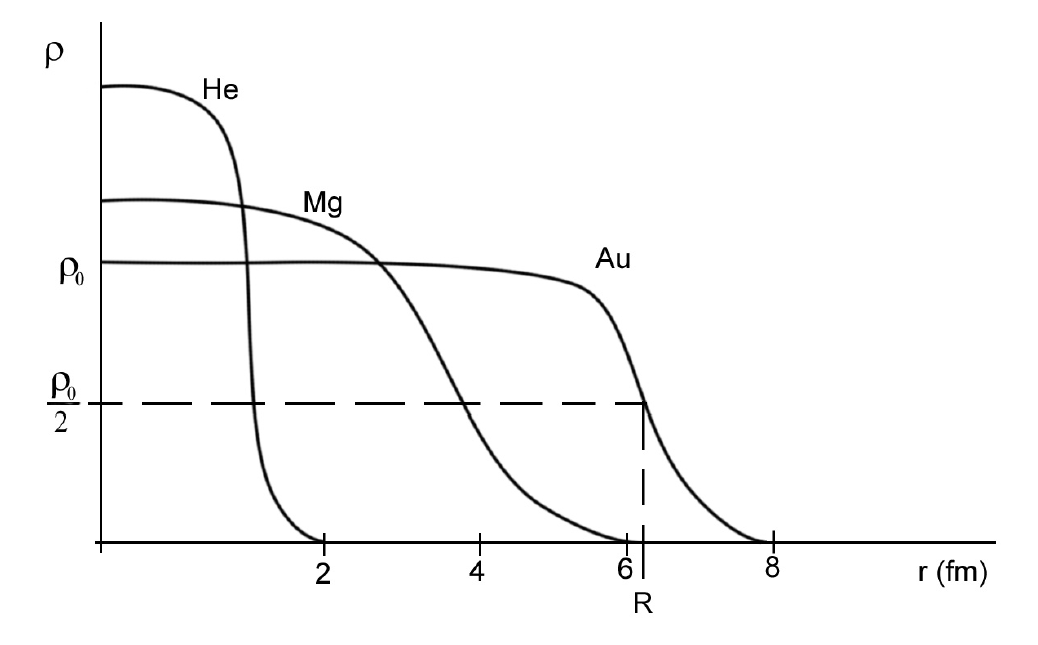
\includegraphics[width=0.8\textwidth]{hustota.png}
	\captionof{figure}{Závislost hustoty náboje na vzdálenosti od středu jádra}		
\end{center}

\section{Hmotnost a vazbová energie}

Hmotnost daného jádra pro daný nuklid $^{A}_{Z} X$ označujeme jako $m(Z,A)$ a vyjádříme ji vztahem
\begin{equation}
m(Z, A) = (A-Z)m_n + Z m_p - \dfrac{B(Z,A)}{c^2}, 
\end{equation}
kde $m_p$ je hmota protonu, $m_n$ hmota neutronu a $B(A,Z)$ je vazbová energie. 

Tato hmotnost souvisí s hmotností atomu $M(Z,A)$ vztahem
\begin{equation}
M(Z,A) = m(Z,A) + Z m_e,
\end{equation}
kde poslední člen vyjadřuje hmotnost $Z$ elektronů. Pokud bychom hmotnost atomu chtěli vyjádřit exaktně, měli bychom brát i vazebné energie elektronů v poli jádra. Ty jsou ale pouze v řádech stovek $\mathrm{eV}$, kdežto atomové jádro má hmotnost $~ 1 ~\mathrm{GeV}$, a tím pádem je lze zanedbat. 

Relativní atomová hmotnost je dána vztahem
\begin{equation}
A_r (^{A} X) = \dfrac{M(^{A} X)}{m_u},
\end{equation}
kde $m_u$ je atomová hmotnostní jednotka, která je určena jako $1/12$ klidové hmotnostiatomu nuklidu $^{12}_{6} C$, tedy platí $m_u = \dfrac{1}{12} M(^{12}_{6}C) = u = 1,66.10^{-27} ~\mathrm{kg}$. Nuklid uhlíku se volí díky tomu, že tvoří spoustu sloučenin, což usnadňuje relativní měření hmotnosti pomocí metody dubletů $\rightarrow$ hmotnostní spektrometry.

Platí také následující vztah
\begin{equation}
E = mc^2 = A_r m_u c^2 = A_r . 931,481 ~\mathrm{MeV}.
\end{equation} 
\begin{itemize}
	\item HMOTNOSTNÍ PŘEBYTEK - je definovaný vztahem $\Delta = A_r - A$, v hmotnostním přebytku jsou zahrnuty vlivy vazbové energie. Např. pokud máme proton a neutron, je součet jejich hmotností jiný, než pokud jsou vázány v deuteronu. 
	\item VAZBOVÁ ENERGIE - je to energie, která se uvolní při vytvoření jádra z jednotlivých nukleonů. Lze ji také označit jako energii, která je (až na znaménko) rovna práci vynaložené k rozdělení jádra na protony a neutrony. Značíme ji $E_v$ a je rovna $E_v = \Delta M c^2$, kde 
\begin{equation}
\Delta M = Z.m_e + m(Z,A) - M(Z,A).
\end{equation}	 
\end{itemize}
Vazbová energie atomů v molekulách se pohybuje řádově v $\mathrm{eV}$, vazbová energie elektronů v atomech nabývá hodnot od několika $\mathrm{eV}$ až po 100 $\mathrm{keV}$ a vazbová energie nukleonů v nejlehčím jádře (deuteronu) přibližně $2,2 ~\mathrm{MeV}$. Procentuální hmotnostní schodek pro atom $^{1}_{1}H$ máme $\Delta M_H = E_{v, H}/c^2 \approx 1,5.10^{-32} ~\mathrm{g}$, což činí asi $1,4.10^{-6} \%$ celkové hmotnosti atomu vodíku.

\subsection{Nukleonová vazbová energie}

Vazebná energie jádra vztažená na jeden nukleon. Značíme ji $\epsilon$ a definujeme ji vztahem
\begin{equation}
\epsilon = \dfrac{E_v}{A}.
\end{equation}

Zajímavá je závislost nukleonové vazbové energie na nukleonovém čísle $A$. 


\begin{center}
	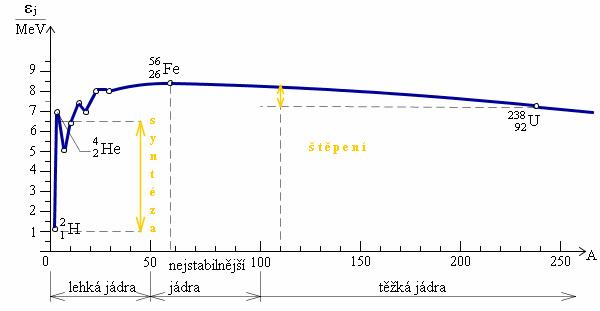
\includegraphics[width=1\textwidth]{vazba.jpg}
	\captionof{figure}{Vazbová energie na nukleon}		
\end{center}

Z grafu vyplývá:
\begin{itemize}
	\item $\epsilon (A)$ rychle roste pro $A \leq 16$,
	\item $\epsilon (A)$ má výrazná maxima pro $A = 4, 12, 16, 20, 24$ (jedná se o sudo-sudá jádra $^{4}_{2}He$, $^{12}_{6}He$, $^{16}_{8}O$, $^{20}_{10}Ne$, $^{24}_{12}Mg$ se stejným počtem protonů a neutronů, která jsou mimořádně stabilní; jejich stabilita je důsledkem slupkové struktury atomových jader), což ukazuje na význam zobecněného Pauliho principu pro nukleony a z toho plynoucí stability jader, která mají celkový počet nukleonů $A= n \alpha$ pro nevelká $n = 1, 2, 3, ...; \alpha$ zde reprezentuje čtyři nukleony částice alfa. 
	\item $\epsilon (A)$ je přibližně konstantní, leží v intervalu $(7,4; 8,8) ~\mathrm{MeV}$ pro všechna jádra s $A > 16$. To tedy znamená, že je pro ně vazbová energie jádra úměrná nukleonovému číslu, $E_v \sim A$. Odtud vyplývá, že nukleon může interagovat jen s omezeným počtem nukleonů. Kdyby tomu bylo při interakci nukleonů stejně jako v systému podrobeném například gravitačním silám, kde každý subjekt interaguje s každým, musela by vazbová energie záviset na počtu různých dvojic nukleonů, tj. mělo by být $E_v \sim \dfrac{1}{2} A(A-1) $. Proto říkáme, že u jaderných sil působících mezi nukleony se projevuje NASYCENÍ. 
	\item $\epsilon (A)$ klesá z maximální hodnoty při $A = 60$ prakticky monotónně až na energii $7,4 ~\mathrm{MeV}$ při $A=238$. Tento pokles je důsledkem vzájemného ELEKTROSTATICKÉHO ODPUZOVÁNÍ PROTONŮ,
	\item Existence maxima $\epsilon (A) $ při $A=60$ (což je nuklid $^{60}_{28}Ni$) je důležitým rozhraním. Z jeho polohy plyne, že jadernou energii lze uvolnit buď při SYNTÉZE, spojení lehkých jader, pokud jejich $A < 60$, anebo při ŠTĚPENÍ těžkých jader na lehčí, přičemž jejich nukleonové číslo musí být větší než 60.
\end{itemize}

Graf $\beta$-stabilních nuklidů můžeme doplnit ještě tím, že přidáme třetí rozměr = hmotnost jádra a vezmeme tak do úvahy všechny nuklidy. V 3D obrazci uděláme řezy v rovinách o konstantním $A$. Průmět jedné z těchto rovin je zobrazen na obrázku $\beta$-stabilních nuklidů $\Rightarrow$ tabulka nuklidů. Typické příklady toho, co se nám v rovinách o konstantním $A$ objeví. Pro lichá $A$ leží v rovině řezu jádra $S-L$ na jedné a jádra $L-S$ na druhé straně od minima, v němž je jádro stabilní vůči rozpadu $\beta$. pro sudé $A$ je to trochu komplikovaější $\Rightarrow$ dostáváme dvě různé křivky, ve spodní leží nejstabilnější jádra $S-S$ a v horní nejméně stabilní jádra $L-L$. 

\begin{center}
	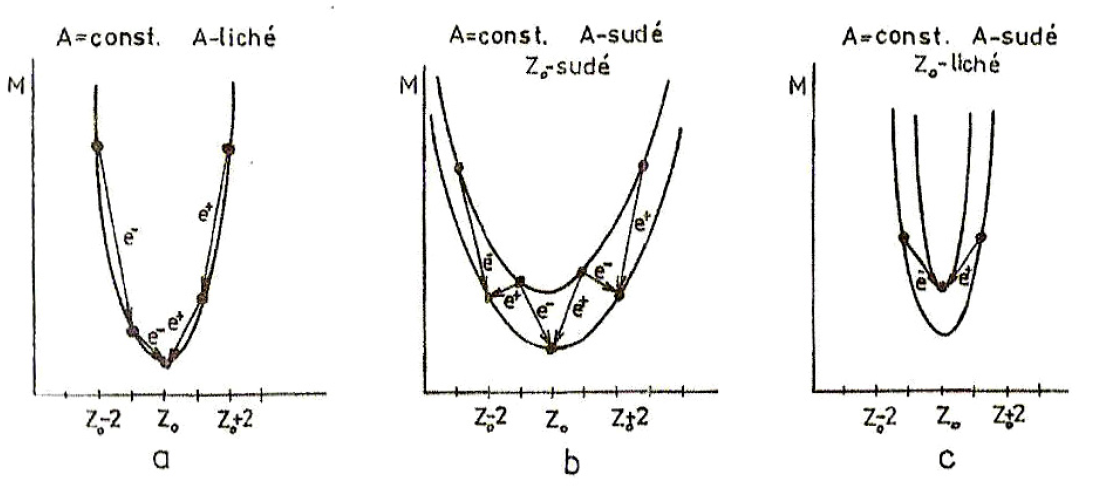
\includegraphics[width=1\textwidth]{rezy.png}
	\captionof{figure}{Řezy uspořádáním všech nuklidů v třírozměrném prostoru ($Z, N, M(A,Z)$) pro konstantní $A$; $a$- nukleonové číslo $A$ je liché, $b$- nukleonové číslo $A$ je sudé a protonové číslo $Z_0$ je sudé, $c$- nukleonové číslo $A$ je sudé a protonové číslo $Z_0$ je liché}		
\end{center}

VAZEBNÁ ENERGIE VZHLEDEM K RŮZNÝM ČÁSTEM ATOMOVÉHO JÁDRA ($E_{v1,2}$). Jádro rozkládáme pouze na dva celky a definujeme tuto energii jako 
\begin{equation}\label{sf6eq:a1}
E_{v1,2} = (m_1 + m_2 - m)c^2 = E_v - E_{v1} - E_{v2}.
\end{equation} 
Je-li $E_{v1,2} < 0$, pak se jádro samovolně rozpadá. Pokud vztah (\ref{sf6eq:a1}) vztáhneme na oddělení pouze jednoho nukleonu z jádra, pak vazbová energie hraje úlohu ionizačního potenciálu dané slupky. Konkrétně se setkáváme se SEPARAČNÍMI ENERGIEMI protonů a neutronů z atomového jádra, platí pro ně vztahy 
\begin{equation}
\epsilon _n = \left[ m_n + m(Z, A-1) - m(Z,A)\right] c^2   ~~~~~~~  \textit{...pro neutron}
\end{equation}
\begin{equation}
\epsilon _p = \left[ m_p + m(Z-1, A-1) - m(Z,A)\right] c^2  ~~~~~~~   \textit{...pro proton}
\end{equation}
Typicky leží separační energie protonů a neutronů v oblasti několik $\mathrm{MeV}$ až 20 $\mathrm{MeV}$. Konkrétní velikost odráží efekty způsobené slupkovou strukturou jádra. Separační energie je energie potřebná k vytržení posledního nukleonu (neutronu). 

Pojem separační energie neutronu ale není definován pro $^{3}_{2}He$. Pokud bychom totiž odtrhli neutron, dostali bychom jádro o dvou protonech, což ale v přírodě nepozorujeme. 

Energii potřebnou navíc k vyjmutí 1 nukleonu ze sudého počtu identických nukleonů nazýváme PÁROVOU ENERGIÍ a zančíme $\delta _n$ či $\delta _p$
\begin{equation}
\delta _n = \epsilon _n (Z,N) - \epsilon _n (Z,N-1) ~~~ \textit{N-sudé $\Rightarrow$ protony}
\end{equation}
\begin{equation}
\delta _p = \epsilon _n (Z,N) - \epsilon _n (Z-1,N) ~~~ \textit{N-liché $\Rightarrow$ neutrony}
\end{equation}

\subsection{Měření hmotnosti jader}

K měření hmotnosti atomů a jader se používají tyto metody:

\begin{itemize}
	\item HMOTOVÁ SPEKTROSKOPIE - přesná, ale časově náročná; pro tuto metodu je nutné mít přesně nakalibrované elektromagnetické pole $\Rightarrow$ experimentálně náročná.
	\item ENERGETICKÁ BILANCE JADERNÝCH REAKCÍ - využívá se znalosti částic vstupujících a vystupujících z jaderné reakce (pokud známe tři hmotnosti ze čtyř). Např. reakce $a + b \rightarrow c + d$, energii reakce dostaneme ze vztahu $Q = (m_a + m_b - m_c - m_d)c^2 = T_c + T_d - T_a - T_d$, přičemž $T_b$ je 0, poněvadž $b$ je terčíková částice. Pokud známe $m_a, m_b$ a $m_c$, dopočítáme $m_d$ ze vztahu $m_d = m_a + m_b - m_c - \Delta m$, kde $\Delta m = Q/c^2 = (T_c + T_d - T_a)/c^2$ lze dopočítat.
	\item ENERGETICKÁ BILANCE RADIOAKTIVNÍCH ROZPADŮ $\alpha$ a $\beta$
	\item STUDIUM ROTAČNÍCH SPEKTER MOLEKUL - Velikost energie rotačních stavů je závislá na momentu setrvačnosti molekuly a ten opět závisí na hmotnostech jader, která se v ní nacházejí. Molekuly, v kterých je atom určitého izotopu nahrazen atomem jiného izotopu téhož prvku, vysílají a případně absorbují fotony, jimž přísluší odlišné frekvence než v původním jádře. To umožňuje určit rozdíl ve hmotnostech jader $\rightarrow$ soudobá mikrovlnná technika $\rightarrow$ malá množství vyšetřovaných látek.
\end{itemize}

Hmotová spektroskopie je z uvedených metod nejdůležitější.


První měření hmotové spektroskopie sestrojili v r. 1918 Aston a Dempster. Základní principy, které byly pro jejich konstrukci použity, jsou aplikovány i v moderních spektrometrech. 

\begin{center}
	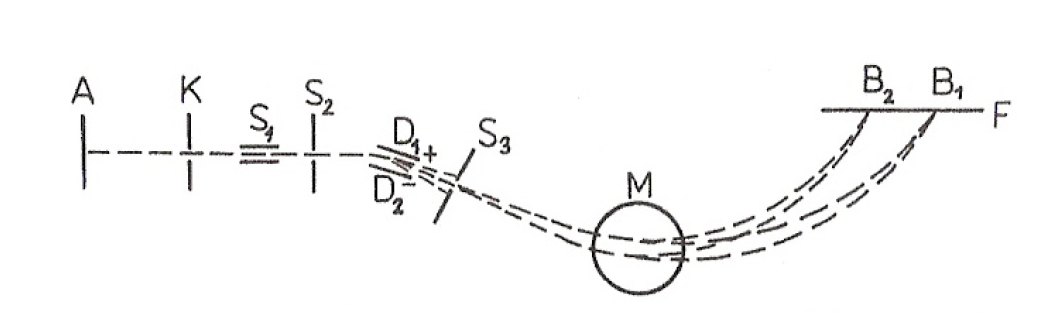
\includegraphics[width=1\textwidth]{aston.png}
	\captionof{figure}{Schéma Astonova spektrometru: $A$- anoda, $K$- katoda, $D_1$ a $D_2$ - elektrody, $M$- střed magnetu, $F$- fotografická deska}		
\end{center}

Celé zařízení je ve skleněné trubici $\rightarrow$ naplněna zkoumaným plynem $\rightarrow$  takový tlak, aby mezi anodou a katodou došlo k ionizaci. Kladně nabité ionty vyvedeny kanálkem $S_1$ a zkolimovány štěrbinou $S_2$. Při přechodu elektrostatickým polem mezi elektrodami $D_1$ a $D_2$ se svazek iontů rozdělí na svazky podle jejich energií $\rightarrow$ štěrbina $S_3$ tak umožní vybrat ionty o prakticky stejné energii. Svazek potom vstupuje do homogenního mag. pole s vektorem mag. indukce kolmým ke směru svazku. V tomto poli je poloměr dráhy iontu úměrný jeho hybnosti $ p= m.v$ $\rightarrow$ využije se při konstrukci aparatury k tomu, aby různě rychlé ionty se stejnou hmotností se zfokusovaly a dopadly do téhož místa $B_1$ na fotografické desce. Ionty s menší hmotností budou mít při stejné energii menší hybnost $p = \sqrt{2mE}$ $\rightarrow$ jejich dráha bude více zakřivení $\rightarrow$ soustředí se do okolí bodu $B_2$. Z polohy bodů $B_1$ a $B_2$ při znalosti konstant aparatury se určí hmotnost iontů $\rightarrow$ a z ní posléze po přidání hmotnosti elektronu a po odečtení ionizační energie dělené $c^2$ se vypočítá hmotnost atomu příslušného nuklidu.

V r. 1913 - Thomson, katodové záření - objev $^{20}Ne , ^{22}Ne$ $\rightarrow$ poprvé viděl izotopy. Měl el. pole + do protisměru mag. pole $\rightarrow$ vidíme parabolickou křivku na destičce $\rightarrow$ selektováné podle poměrů nábojů a hmotností.

V r. 1918 - Dempster : rychlostní separátor, štěrbina - el. pole + mag. pole $\rightarrow$ vybereme část svazku s danou rychlostí. Projdou jen částice s rychlostí $v_0 = E/B$.

 
Soudobé spektrometry mají tři části:
\begin{itemize}
	\item IONTOVÝ ZDROJ - zisk iontů, nejen klasickými metodami, ale i za pomoci vysokofrekvenčního pole
	\item ENERGETICKÝ SELEKTOR - buď elektrostatický selektor nebo rychlostní elektromagnetický
	\begin{itemize}
		\item ELEKTROSTATICKÝ SELEKTOR - pracuje podobně jako Astonův se dvěma elektrodami $D_1$ a $D_2$, které však nyní mají tvar kruhového oblouku a jsou zdrojem radiálního elektrického pole o intenzitě $E$, která vybírá z iontů o náboji $q$ a o různých energiích právě ty, které se pohybují po dráze o poloměru $r$ a mají energii
		\begin{equation}
		\dfrac{1}{2} m v^2 = \dfrac{1}{2} qrE.
		\end{equation} 
		\item RYCHLOSTNÍ ELEKTROMAGNETICKÝ - využívá možnosti, že v elektromagnetickém poli, ve kterém bude platit pro intenzitu $\vec{E}$ a indukci $\vec{B}$ vztah $\vec{E} = \vec{B} \times \vec{v}$, kde $\vec{v}$ je rychlost iontu, bude Lorentzova síla působící na iont
		\begin{equation}
		\vec{F} = q(\vec{E} + \vec{v} \times \vec{B}) \equiv 0.
		\end{equation}
		
		\begin{center}
			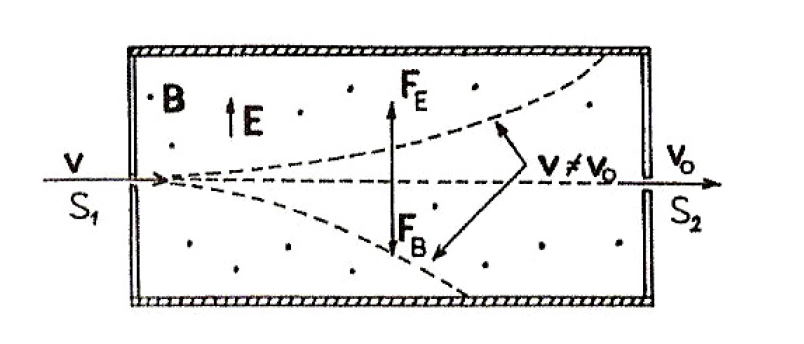
\includegraphics[width=0.6\textwidth]{selektor.png}
			\captionof{figure}{Princip rychlostního selektoru.}		
		\end{center}
		
		$\vec{F_E}$ je síla vyvolaná el. polem, jehož intenzita $\vec{E}$ leží v rovině dráhy, $\vec{F_B}$ je síla vyvolaná mag. polem, jehož vektor indukce $\vec{B}$ je kolmý k rovině dráhy. Rychlost $\vec{v_0}$ je rychlost, pro kterou je splněna podmínka $\vec{F_E} + \vec{F_B} = 0$. Úhel $\beta$ je určen poměrem maximálního průměru štěrbiny $S_{2}$ k její vzdálenosti od štěrbiny $S_1$.
		
		To znamená, že iont, který bude splňovat tuto podmínku, se bude pohybovat přímočaře v daném poli, zatímco ionty, který ji nesplní, z této dráhy vybočí a může být zachycen. Za výstupní štěrbinou dostáváme ionty s rychlostmi $v \in (v_0, v_0 \cos \beta)$, kde $v_0 = E/B$ a úhel $\beta$ je určen geometrií výstupní štěrbiny a charakterizuje kvalitu selektoru. Princip rychlostního selektoru lze pochopit z obrázku.
	\end{itemize}
	\item MAGNETICKÝ ANALYZÁTOR - s elektrickým registračním zařízením snímajícím spektrum hmotností u spektrometrů a s fotografickým nebo na polohu citlivým  elektrickým zařízením měřícím toto spektrum u spektrografů.
\end{itemize}

\begin{center}
	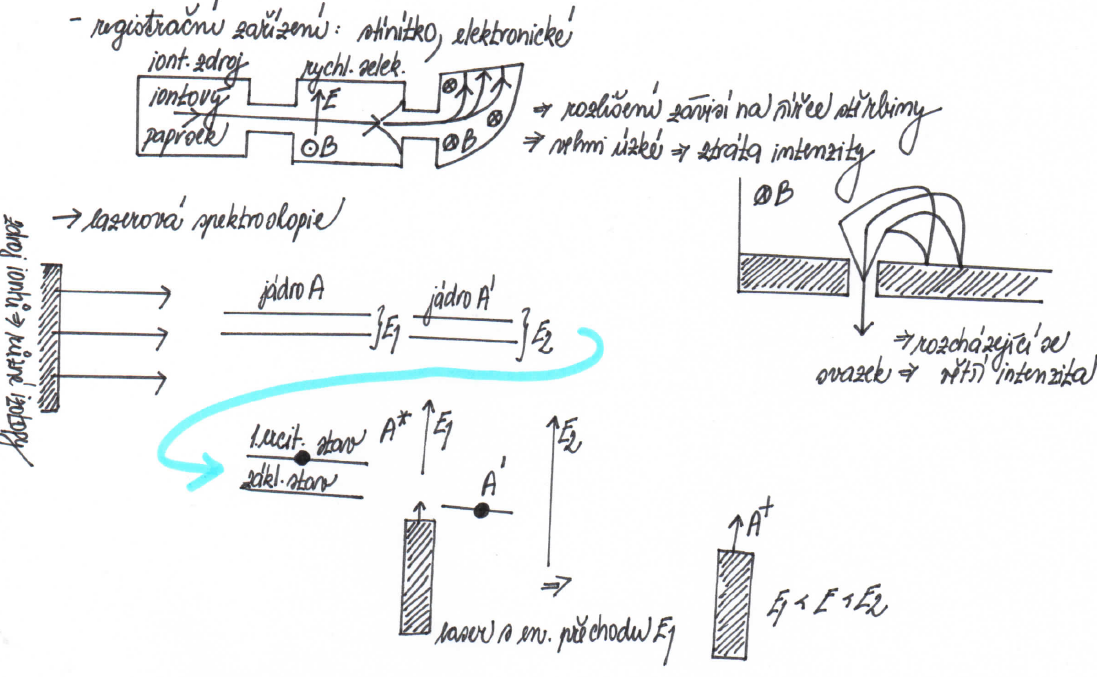
\includegraphics[width=1\textwidth]{analyz.png}
	\captionof{figure}{Magnetický analyzátor}		
\end{center}

Soudobé hmotové spektrometry umožňují určovat hmotnosti iontů s relativní chybou menší než $10^{-7}$. Nejpřesnější měření se dosahují tzv. METODOU DUBLETŮ, při níž se měří rozdíl hmotnosti iontů, které by se měly zobrazit v hmotovém spektrometru stejně, kdyby jejich hmotnost byla násobkem počtu nukleonů, které obsahují. Kvůli této metodě byl vybrán nuklid $^{12}_{6}C$ za základ pro definici atomové hmotnostní jednotky.

\subsection{Tabulka nuklidů}

Známé hmotnosti asi 2000 nuklidů (265 stabilních) lze roztřídit na základě toho, co již víme. 
\begin{itemize}
	\item nuklidy stabilní vůči $\beta$ rozpadu - zcela stabilní nuklidy a nestabilní nuklidy nepodléhající radioaktivnímu rozpadu $\beta$ $\rightarrow$ asi 350 $\rightarrow$ LINIE STABILITY $\beta$, kde se nacházejí $\beta$ stabilní nuklidy,
	\item jádra ležící pod linií stability (při pevném $Z$ mají vyšší $N$) $\rightarrow$ rozpadají se samovolně pomocí $\beta ^-$,
	\item nad linií stability se jádra rozpadí pomocí $\beta ^+$, tato jádra jsou také nestabilní vůči ZÁCHYTU.
\end{itemize}

\begin{center}
	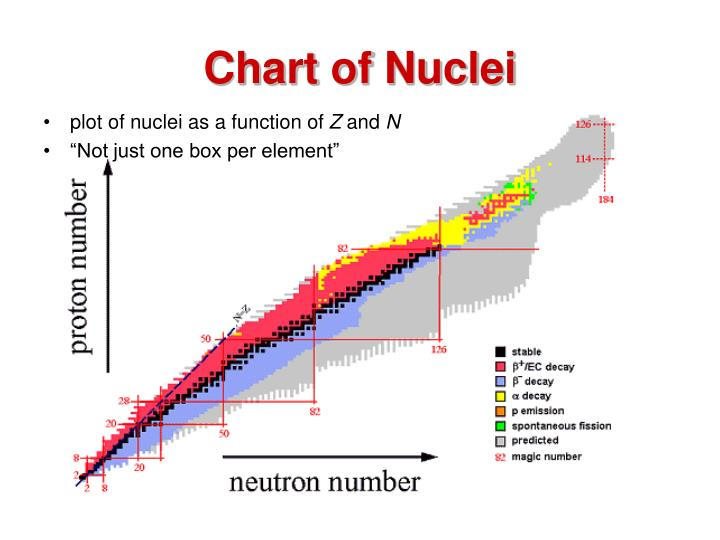
\includegraphics[width=1\textwidth]{chart_nuclei.jpg}
	\captionof{figure}{Tabulka nuklidů}		
\end{center}

Pro malý počet nukleonů jsou stabilní ta jádra s $N=Z$ do $N=30$. Se zvětšováním $A$ se pás stability odklání od této přímky směrem k většímu počtu neutronů $\rightarrow$ důvody pro toto chování jsou skryty v působení Coulombovy síly. Pokud je v jádře více protonů, roste Coulombické odpuzování, které musí být kompenzováno potřebným přebytkem neutronů. 

V oblasti olova ($Z=82, N=126$) se pás $\beta$-stability jader přerušuje a všechna těžší jádra jsou nestabilní. Z tabulky nuklidů lze také zjistit, že nejvíce stabilních nuklidů má sudé jak protonové, tak i neutronové číslo. Tato skutečnost svědčí o tendenci jaderných sil párovat nukleony stejného typu, jelikož v páru jsou nukleony vázány silněji. 

\section{Způsoby uvolňování energie}

Energii lze uvolnit převedením systému, který je méně vázán, do systému, jehož komponenty jsou vázány silněji. Můžeme to udělat pomocí jaderné syntézy, štěpení těžkých atomových jader, či anihilací.

Můžeme tak však činit i chemickým procesem spalování, např. $C + O_2 \rightarrow CO_2 + Q$, kde uvolněná energie $Q = 94 \mathrm{kJ/mol} = 246,9.10^{16} ~\mathrm{MeV/mol}$. Uvolněná energie při vzniku jedné molekuly $CO_2$ je $E_v = \Delta M c^2 = Q/N_A = 4,1 ~\mathrm{eV}$, přičemž $N_A$ je počet částic v jednom molu. Hmotnost jednoho molu $CO_2$ je $44 g$, takže podíl $\Delta M/M \sim 10^{-10}$. 

Například pro proces $H_2 + \dfrac{1}{2}O_2 \rightarrow H_2 O$ je podíl $\Delta M/M \sim 1,5.10^{-10}$. Takže relativní změna hmotnosti při spalování je $\Delta M/M \sim 10^{-10}$.

Uvolnit energii lze i rekombinací $e^- + p \rightarrow H$, kde $E_v = \left[ m_e + m_p - M\left( ^{1}_{1} H\right) \right] c^2 = 13,6 ~\mathrm{eV}$. Relativní změna hmotnosti při rekombinaci je $\Delta M/M \sim 10^{-8}$. 

\subsection{Jaderná fúze}

Při jaderné fúzi vezmeme dvě slaběji vázaná jádra a spojíme je v jedno. Poprvvé ji formuloval v r. 1939 Bethe hypotézou, že jaderné reakce dodávají energii k pohonu Slunce. Provázal tak astrofyziku s jadernou fyzikou. Na Slunci probíhají dva cykly, přičemž v obou se vytvářejí z protonů při působení silné, elektromagnetické a slabé interakce jádra helia, částice $\alpha$. Zde jsou oba cykly popsány:

\begin{itemize}
	\item PROTON-PROTONOVÝ CYKLUS (p-p cyklus) se realizuje jako	
\begin{equation}
^{1}_{1} H + ^{1}_{1} H \rightarrow ^{2}_{1} H + e^+ + \nu _e + 0,4 ~\mathrm{MeV},
\end{equation}
\begin{equation}
^{2}_{1} H + ^{1}_{1} H \rightarrow ^{3}_{2} He + \gamma + 5,5 ~\mathrm{MeV},
\end{equation}
\begin{equation}
^{3}_{2} He + ^{3}_{2} He \rightarrow ^{4}_{2} He + 2 ^{1}_{1} H  + 12,9 ~\mathrm{MeV},
\end{equation}
po uzavření celého procesu tedy máme: $4p \rightarrow ^{4}_{2} He + 2 e^+ + 2 \nu_e + 2 \gamma + 26,7 ~\mathrm{MeV}$. Proton-protonový cyklus dává výtěžek $\Delta M /M = 6,6.10^{-3}$.

   \item UHLÍKO-KYSLÍKOVÝ CYKLUS je složený z reakcí
\begin{equation}
^{12}_{6} C + ^{1}_{1} H \rightarrow ^{13}_{7} N + \gamma +  1,93 ~\mathrm{MeV},
\end{equation}   
\begin{equation}
^{13}_{7} N  \rightarrow ^{13}_{6} C + e^+  + \nu _e  +  1,2 ~\mathrm{MeV},
\end{equation} 
\begin{equation}
^{13}_{6} C + p \rightarrow ^{14}_{7} N + \gamma +  7,6 ~\mathrm{MeV},
\end{equation} 
\begin{equation}
^{14}_{7} N + p \rightarrow ^{15}_{8} O + \gamma +  7,4 ~\mathrm{MeV},
\end{equation} 
\begin{equation}
^{15}_{8} O \rightarrow ^{15}_{7} N + e^+ + \nu _e + \gamma +  1,7 ~\mathrm{MeV},
\end{equation} 
\begin{equation}
^{15}_{7} N + ^{1}_{1} H \rightarrow ^{12}_{6} C + \alpha +  5 ~\mathrm{MeV},
\end{equation}
po uzavření cyklu tedy máme proces: $4p \rightarrow  ^{4}_{2} He + 2 e^+ + 2 \nu_e + 3 \gamma + 26 ~\mathrm{MeV}.$
\end{itemize}

\begin{figure}
	\begin{minipage}[c]{0.4\linewidth}
		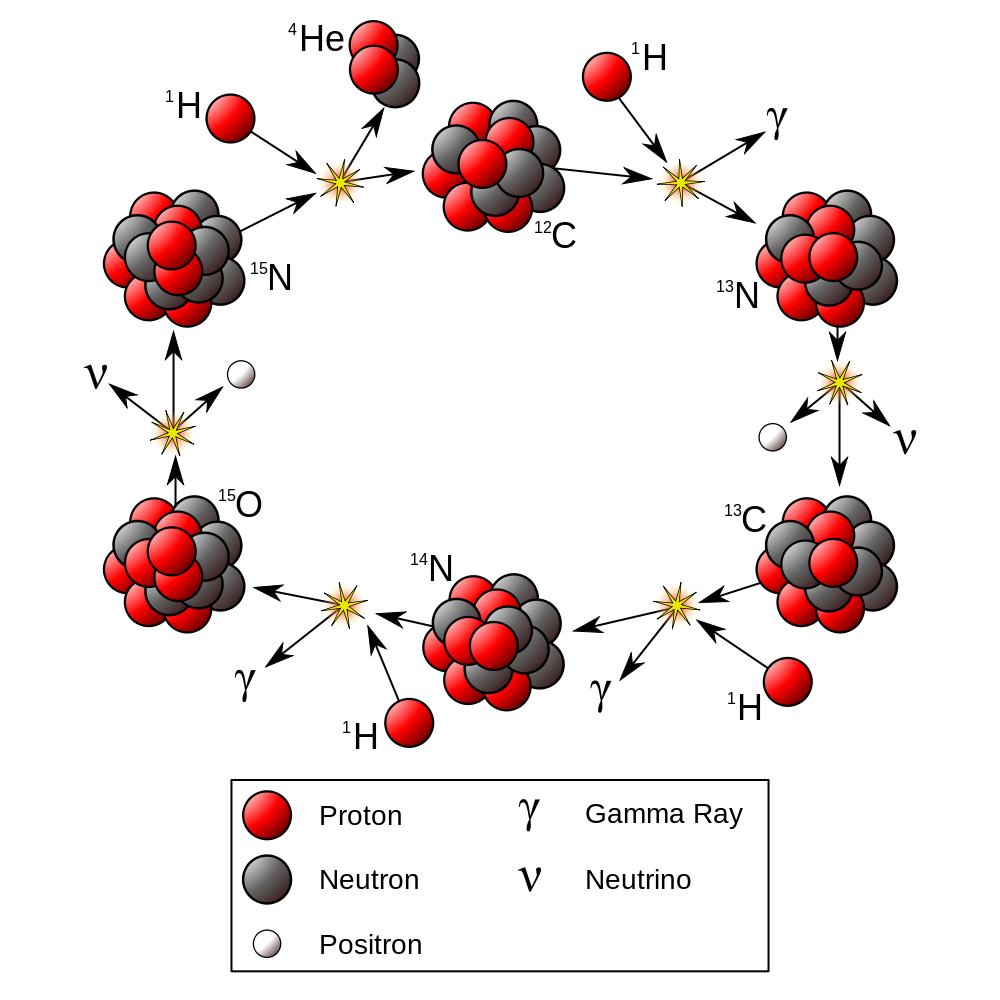
\includegraphics[width=\linewidth]{CNO_cyklus.png}
		\caption{CNO cyklus}
	\end{minipage}
	\hfill
	\begin{minipage}[c]{0.4\linewidth}
		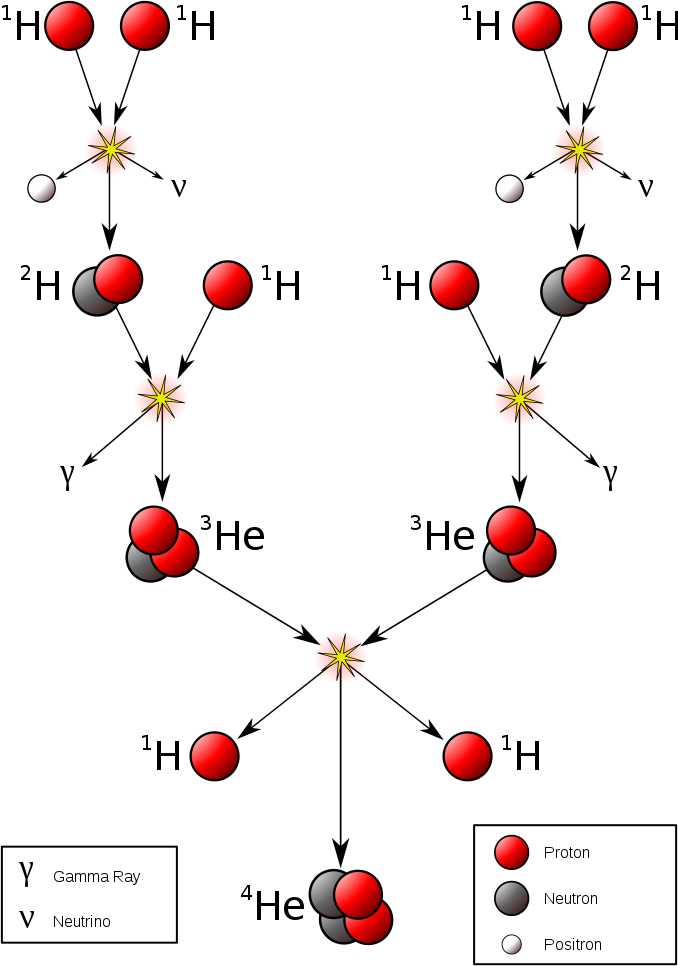
\includegraphics[width=\linewidth]{proton_proton.png}
		\caption{Proton-protonový cyklus}
	\end{minipage}
\end{figure}

Abychom ale mohli realizovat jadernou syntézu, je nutno překonat Coulombické odpuzování mezi jádry. To se děje díky zvýšení teploty na velmi vysokou hodnotu přibližně $10^7 ~\mathrm{K}$, čemuž odpovídá střední kinetická energie protonů přibližně $2 ~\mathrm{keV}$. Jelikož je to ale pouze střední kinetická energie, relativně mnoho protonů bude mít dostatečně vysokou energii, rovnou řádově několika $\mathrm{MeV}$, k tomu, aby protony pronikly Coulombickou bariérou a došlo tak k vlastní jaderné reakci.

Slunce má na svém povrchu teplotu $\sim$ $10^6 ~\mathrm{K}$, uvnitř pak $\sim$ $10^7 ~\mathrm{K}$ a každou sekundu se v něm promění přibližně $0,5$ miliardy tun vodíku v hélium. Navíc jeho výkon je $3,8.10^{26} ~\mathrm{W}$.

Exotermické reakce, které vedou k syntéze, jsou dnes dobře prozkoumány. Problémem však zůstává kontrola celého procesu v prakticky využitelném rozsahu. Z exotermických reakcí se slibnými z hlediska aplikací v množných energetických zdrojích v budoucnosti jeví např. tyto reakce:

\begin{equation}
d + d \rightarrow ^{3}_{2} He + n + 3,25 ~\mathrm{MeV},
\end{equation} 
\begin{equation}
d + d \rightarrow ^{3}_{1} H + p + 4 ~\mathrm{MeV},
\end{equation} 
\begin{equation}
p + ^{7}_{3} Li \rightarrow \alpha + \alpha + 17 ~\mathrm{MeV},
\end{equation} 
\begin{equation}
d + t \rightarrow \alpha + n + 17,6 ~\mathrm{MeV}.
\end{equation} 

Největší uvolněnou energii připadající na jeden nukleon dává poslední z nich, $Q/A$ je u ní totiž $3, 52 ~\mathrm{MeV}$ a to je hodnota čtyřnásobně vyšší, než se získává štěpením jádra $^{235}_{92} U$. 

\subsection{Štěpení těžkých atomových jader}

Štěpná reakce je reakcí, při které se atomové jádro rozštěpí, rozdělí na dvě nebo více jader. Štěpení na dvě jádra je mnohem pravděpodobnější než štěpení na více jader.

Projektil o dostatečně vysoké energii může rozštěpit jakékoliv jádro s protonovým číslem $Z \geq 2$, a proto štěpná reakce nepředstavuje zcela mimořádný děj, který vždy probíhá v souladu se zákony zachování. Čím má jádro vyšší hmotnostní číslo $A$, tím je pravděpodobnost štěpné reakce vyšší.
\begin{itemize}
	\item štěpení jader uranu $U$
\end{itemize}  
Používá se běžně v současné energetice. Základní štěpná reakce, která  umožňuje aplikace uranu, je exotermická reakce, probíhající po absorbci tepelného neutronu (neutrony je nutno zpomalit moderátorem) v jádře $^{235}_{92} U$:
\begin{equation}
n + ^{235}_{92} U \rightarrow ^{A_1}_{Z_1} X_1 + ^{A_2}_{Z_2} X_2 + kn + m \gamma,
\end{equation}
kde zákon zachování náboje dává $Z_1 + Z_2 = 92$ a zákon zachování nukleonů $A_1 + A_2 + k = 236$ a kde $k = 2, 3$ a $m = 1, 2, ..., r$. V reakci navíc kromě dvou jader, tzv. odštěpků, vznikají dva nebo tři neutrony a tvrdé fotony $\gamma$. Vzniklá jádra mají obecně přebytek neutronů, což je způsobeno tím, že mateřská jádra jsou před štěpením těžká a o těch víme, že mají přebytek neutronů. Při štěpení se vyzařují volné neutrony a odštěpky jsou beta-radioaktivní $\rightarrow$ cílem beta-radioaktivity u odštěpků je přiblížit se linii stability. Neutrony takto vyslané se zpožděním za neutrony z vlastního štěpení = zpožděné tvoří necelé procento z celkového počtu neutronů vzniklých při štěpení a mají poměrně malou kinetickou energii $< 1 ~\mathrm{MeV}$. Bez zřetele na malý podíl zpožděných neutronů v celkovém počtu okamžitých neutronů mají právě tyto neutrony při práci jaderných reaktorů velmi důležitý význam - umožňují řídit průběh řetězové reakce. 

\begin{center}
	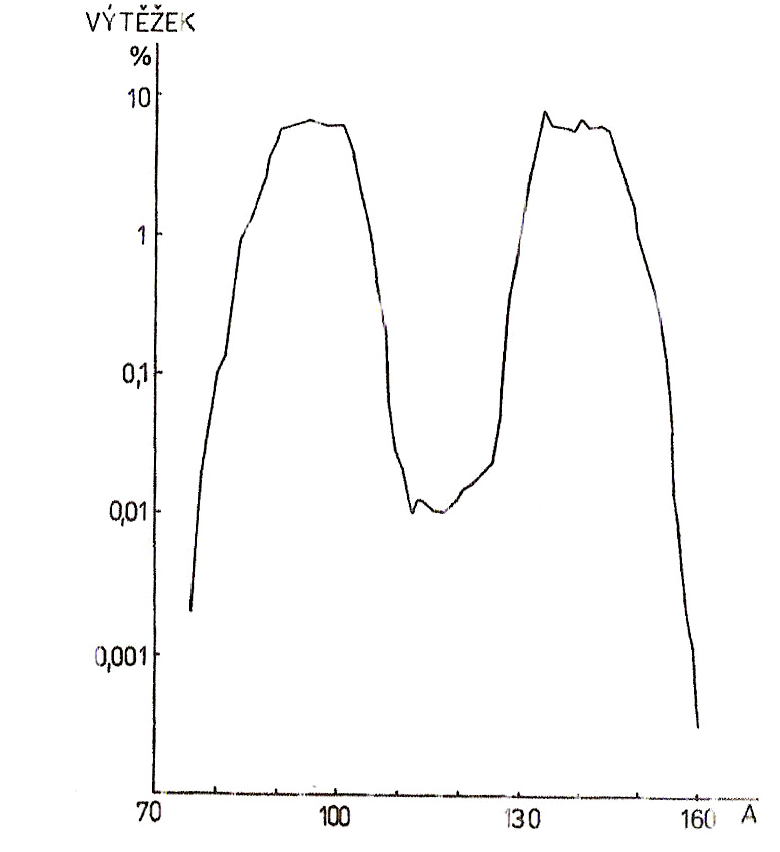
\includegraphics[width=0.5\textwidth]{fragment.png}
	\captionof{figure}{Rozdělení štěpných fragmentů pro nuklid $^{235}_{92}U$.}		
\end{center}

Celková uvolněná energie je dána jako součet energie $Q_f$ uvolněné štěpením a energie $Q_{\beta _i}$ uvolněné při $\beta$-rozpadech produktů a je rovna
\begin{equation}
Q = Q_f + \sum_{i} Q_{\beta_i} \approx 195 ~\mathrm{MeV}.
\end{equation}

Při štěpné reakci se na jeden nukleon uvolní zhruba $7$-krát méně energie než při syntéze jader, protože
\begin{equation}
\dfrac{(\Delta M/M)_{synteza}}{(\Delta M /M)_{stepeni}} = \dfrac{6,6.10^{-3}}{8,9.10^{-4}} \approx 7,4.
\end{equation}
Obě jádra = fragmenty (odštěpky), které vznikají při štěpení, patří do relativně širokého spektra fragmentů. Jejich známá nukleonová čísla $A$ pokrývají všechny možné hodnoty v intervalu (76, 160) tak, aby počet přislušných dvojic dal vždy číslo $A = 234$ nebo $A = 233$. Jejich pravděpodobné zastoupení má dvě maxima typická i pro ostatní štěpné reakce. U nuklidu $^{235}_{92} U$ tato maxima leží v okolí $A = 95$ a $A = 139$.

Změřené šířky nízkoenergetických rezonancí v účinném průřezu štěpení uranu $^{235}_{92} U$ jsou přibližně $0,1 ~\mathrm{eV}$. Štěpení se děje v čase $\tau_f = \hbar /\Gamma_f \approx 10^{-14} ~\mathrm{s}$ po absorbci neutronu.

Původ štěpné reakce: jádro $^{235}_{92} U$ vytvoří po absorbci neutronu metastabilní jádro $\rightarrow$ díky kvantovým oscilacím se jádro silně deformuje (protáhlý tvar) $\rightarrow$ repulsivní Coulombické síly roztrhnou jádro na dvě části (někdy i tři a více).Významnou roli hraje poměr mezi jadernými silami krátkého dosahu a Coulombickými silami dlouhého dosahu a také tunelový jev při průchodu fragmentů potenciálovou bariérou. 

\subsection{Anihilace}

Při anihilaci se setkávají částice s antičásticemi, které spolu zreagují a zaniknou za vzniku jiných částic, převážně fotonů (elektromagnetická interakce) či mezonů (silná interakce). Při anihilaci vždy platí zákony zachování energie, hybnosti, ... . Součet aditivních kvantových čísel před anihilací a po anihilaci je roven nule. Uveďme např. proces
\begin{equation}
e^+ + e^- \rightarrow q + \overline{q},
\end{equation}
kde se celá klidová energie pozitronu a elektronu přemění na záření, tj. hmotnostní deficit je $\Delta M/M \sim 1$. Proces anihilace hmoty s antihmotou se jeví jako ideální zdroj energie $\rightarrow$ \glqq palivo\grqq ~lze spotřebovat beze zbytku (u současných reaktorů se spotřebuje pouze několik procent paliva). \glqq Výhřevnost\grqq ~anihilačního paliva je 100-1000-krát větší než u jaderného paliva a to je asi $10^7$-krát \glqq výhřevnější\grqq ~než chemické palivo. Anihilace však nemá jako zdroj energie praktický význam $\rightarrow$ pro vytvoření vhodných podmínek pro anihilaci je zapotřebí mnohem více energie, než se při ní uvolní. Náročné je také vytvořit stabilnější antihmotu (antiprotony, antineutrony $\rightarrow$ antijádra $\rightarrow$ antiatomy).  


\section{Spin, izospin, parita jádra}

Představme si (jako v kvantové mechanice), že vektor spinu vykonává precesi kolem jedné osy (např. $z$). Spektrum operátoru spinu $\hat{S}_z$ je diskrétní a jeho vlastní hodnoty jsou $\pm \hbar$. Časově nezávislé jsou i vlatsní funkce $\hat{S} ^2$.

V případě jádra je situace složitější, protože je složeno z nukleonů a každý nukleon má vlastní spin $\rightarrow$ spin jádra bude složeninou všech nukleonů. Spin jádra budeme označovat symbolem $I$ $\rightarrow$ od teď budeme o spinu mluvit jako o vlastní hodnotě příslušného operátoru. Hodnoty spinu nebudou jen dvě (jako u fermionů), ale bude jich celá řada. Ostrých hodnot nabývá spin pouze v jednom směru $\rightarrow$ kterou z těchto hodnot $I_z$ ale máme použít pro klasifikaci vnitřního stavu jádra.

SPINEM JÁDRA $I$ budeme rozumět nejvyšší možnou hodnotu z $2I + 1$ možných hodnot z-ové komponenty vektoru spinu $\vec{I}$, platí tedy
\begin{equation}
(I_z)_{max} = I \hbar.
\end{equation}

Projekce spinu se měří v jednotkách $\hbar$. Experimentálně bylo zjištěno několik poznatků:
\begin{itemize}
	\item Pokud $A$ je SUDÉ $\Rightarrow$ $I$ je CELÉ ČÍSLO a taková jádra se chovají jako BOSONY, 
	\item Pokud $A$ je LICHÉ $\Rightarrow$ $I$ je POLOČÍSELNÉ a jádra se chovají jako FERMIONY,
	\item SUDO-SUDÁ JÁDRA mají spin $I = 0$, platí u nich totiž tzv. PÁROVÝ EFEKT - nukleony se spárují do dvojic s opačným spinem a celkový spin se vyruší,
	\item jádra SUDO-LICHÁ nebo LICHO-SUDÁ mají POLOČÍSELNÝ SPIN,
	\item jádra LICHO-LICHÁ mají spin NENULOVÝ, CELOČÍSELNÝ, KLADNÝ,
	\item Hodnoty spinu jader v základním stavu leží v intervalu $\langle 0; 8\rangle$.
\end{itemize}

Důležitou vlastností jádra je, že vektor $I$ je jedinou nezávislou vektorovou charakteristikou jádra. Všechny ostatní vektorové a tenzorové veličiny lze vyjádřit její pomocí.

Libovolná veličina $A$ je tak úměrná spinu: $A = \alpha I$.

Libovolná veličina $B$, která je symetrickým tenzorem s nulovou stopou ($\Sigma_{i} B_{ij} = 0$), má tvar
\begin{equation}
B_{ij} = \beta \left( I_i I_j + I_j I_i - \dfrac{2}{3} \delta _{ij} I(I + 1)\right) .
\end{equation}
Odtud plyne, že částici s nulovým spinem nemohou popsat klasické vektory - pouze axiální pseudovektory. Jádra a částice mohou mít pouze magnetický dipólový moment (nikoliv elektrický) a elektrický kvadrupólový moment (ne magnetický).

\subsection{Parita}

Paritu jádra udáváme vždy v jeho základním stavu a nahlížíme na ni jako na vnitřní paritu. Parita SUDO-SUDÝCH JADER je KLADNÁ, u ostatních jader může být jak kladná tak záporná. I ve fyzice atomového jádra paritu symbolizujeme jako horní index u spinu jádra nebo částice, tj. $I^+$ (pro sudo-sudá jádro tak bude spin-parita $0^+$). Parita excitovaných stavů jádra může být shodná s paritou jádra v základním stavu $\Rightarrow$ excitované stavy s normální paritou. V opačném případě jde o excitované stavy s nenormální paritou. U většiny jader mají stavy s nenormální paritou vyšší energii než stavy s normální paritou. Mezi základním stavem a prvním stavem s nenormální paritou se obvykle nachází několik stavů s normální paritou. 

Využijeme-li slupkového modelu, bude parita jádra určena vztahem
\begin{equation}
P = \Pi _{i = 1} ^{A} (-1)^{l_i},
\end{equation}
kde $l_i$ je kvantové číslo momentu hybnosti i-tého nukleonu. Jedním z důležitých důsledků existence parity stavů atomového jádra je např. to, že elektrický dipólový moment jádra musí být nulový. Vlnová funkce jádra nemůže změnit při inverzi souřadnic  (na kterých závisí) svou absolutní hodnotu, neboť je to funkce pro dva systémy fermionů, pro každý z nich platí Pauliho vylučovací princip. Proto hustota pravděpodobnosti pro rozložení náboje v jádře, která je úměrná kvadrátu absolutní hodnoty této vlnové funkce, se chová jako funkce sudá, tj. $\rho (\vec{r}) = \rho (- \vec{r})$, a tedy elektrický dipólový moment, který je dán integrálem 
\begin{equation}
\vec{d} = e \int_V \vec{r}_{\rho} (\vec{r}) dV,
\end{equation}
je roven nule (integrand je lichý). Z tohoto důvodu lze elektrické vlastnosti atomového jádra vedle jeho celkového náboje detailněji popsat až s pomocí elektrického kvadrupólového momentu. 

\subsection{Izospin (Izotopický spin)}

Nukleonům připisujeme izospin $T = 1/2$ a jeho projekce $T_z$ je rovna $+ 1/2$ pro protony a $-1/2$ pro neutrony. Z proton-neutronové stavby atomového jádra ihned plyne, že izospin jádra, který se určuje podle pravidel pro skládání momentů hybnosti, je roven $n = 0, 1, 2, ...$ pro $A$ SUDÉ a $n + 1/2; n = 0, 1, 2, ...$ pro $A$ LICHÉ. Relativně široký interval možných hodnot $n$ se dá omezit, využijeme-li představ slupkového modelu jádra. Izospiny jednotlivých nukleonů se spárují a poslední nespárované nukleony určí celkový izospin jádra. 

Např. zrcadlová jádra $^{7}_{4} Be$ a $^{7}_{3} Li$  mají 3 spárované protony a 3 neutrony $\rightarrow$ $T = 0$ a poslední nukleon dává $T = 1/2$ pro celé jádro. Tutíž $Be$ má $T=1/2$ a $T_z = +1/2$ a $Li$ má $T =1/2$ a $T_z = -1/2$.

Izospin je ale daleko výhodnější určovat experimentálně $\rightarrow$ zjišťování, která z povolených hodnot celkového izospinu $T$  se skutečně v daném jádře realizuje a tím i určit, v kolika nábojových stavech s toutéž energií, paritou a spinem se může daná soustava nukleonů nacházet. Projekce celkového izospinu jádra $T_z$ je bezprostředně dána jako součet projekcí izospinů jednotlivých nukleonů
\begin{equation}
T_z = \dfrac{1}{2} (Z - N).
\end{equation}

Odtud bezpečně určíme jen dolní mez pro hodnotu celkového izospinu $T$. K celkovému určení izospinu musíme přejít k experimentálním údajům. Vezmeme např. jádra s $A=10$:  $^{10}_{4} Be$,  $^{10}_{5} B$ a  $^{10}_{6} C$. Prvnímu excitovanému stavu jádra  $^{10}_{5} B$ s $T_z = 0$ přísluší celková energie, která je přibližně rovna klidové energii základního stavu jader  $^{10}_{4} Be$ s $T_z = -1$ a  $^{10}_{6} C$ s $T_z = +1$. Protože i jejich spiny a parity jsou jsou shodné, tvoří tyto tři stavy izospinový triplet a je jim třeba připsat $T=1$. Základní stav jádra  $^{10}_{5} B$
 s $T_z = 0$ nemá žádného partnera, a proto mu připisujeme $T = 0$. Stejný rozbor můžeme udělat u ostatních stavů těchto jader, abychom určili jejich izospin. Nábojové multiplety tohoto druhu lze nalézt i v mnoha dalších případech. Příslušné hodnoty izospinu tu jsou $T = 1/2$ u lichých zrcadlových jader a dále $1, 3/2, 2$. Pro těžší jádra s $A > 50$ izospinový formalismus ztrácí svůj praktický význam, neboť tam je elektrostatická repulze jádra již příliš silná.
 
Možnost klasifikovat izospinové stavy jader dala podnět k vyslovení hypotézy o nábojové nezávislosti jaderných sil $\rightarrow$ jaderné síly sice závisejí na izospinu, ale nikoliv na jeho složce. Dále z této hypotézy plyne, že v procesech, které jsou určeny silnými interakcemi, se zachovává izospin $T$ i jeho složka $T_z$. 

Naproti tomu v reakcích, které probíhají pod vlivem elektromagnetické interakce se bude zachovávat pouze projekce izospinu $T_z$, celkový izospin se obecně zachovávat nebude. Velmi dobře jsou známy radiační přechody $\gamma$ mezi stavy s různým izospinem $T$. Při radioaktivních dějích provázených vyzářením elektronů a pozitronů se nezachovává ani $T_z$, neboť se při nich mění neutron v proton nebo proton v neutron. Stejně je tomu při zachycení elektronu v jádře.  





\subsection{Magnetický dipólový moment jádra}

Elektron obíhající kolem kladně nabitého jádra vytvoří proudovou smyčku a pro proud podle klasické elektrodynamiky máme vztah
\begin{equation}
I = \dfrac{dQ}{dt} = \dfrac{e}{T} = e \nu,
\end{equation}
kde $\nu$ je frekvence. Velikost magnetického dipólového momentu elektronu pohybujícího se po kruhové dráze lze napsat jako 
\begin{equation}
\mu = IS = \pi R^2 e \nu = \dfrac{m_e}{m_e} \pi R^2 e \nu = \dfrac{e}{2 m_e} m_e R v = \dfrac{e}{2 m_e}l,
\end{equation}
kde $l$ je orbitální moment hybnosti elektronu.

Magnetický dipólový moment je tedy spojen s orbitálním pohybem nabité částice $\rightarrow$ orbitální moment hybnosti. Existuje také vlastní moment hybnosti částice, který se nazývá spinový. V případě atomového jádra musíme zahrnout ještě FAKTOR JÁDRA $g$ a nahradit orbitální moment hybnosti $l$ spinem jádra $I$. Potom je MAGNETICKÝ DIPÓLOVÝ MOMENT JÁDRA dán vztahem
\begin{equation}
\vec{\mu} = g \dfrac{e}{2 m_p} \vec{I} = \gamma \vec{I},
\end{equation} 
kde $\gamma$ je gyromagnetický poměr - veličina, která udává poměr magnetického a mechanického momentu. Jedna komponenta ($\mu _z$) je kvantována
\begin{equation}
\mu _z = g \dfrac{e}{2 m_p} I_z = g \dfrac{e \hbar}{2 m_p} m_I = g \mu_N m_I,
\end{equation}
kde $m_I = \vec{I} /\hbar$, $\mu _N = e \hbar /2 m_p = 5, 05.10^{-27} ~\mathrm{JT^{-1}}$ je JADERNÝ (NUKLEÁRNÍ) MAGNETON. Ve srovnání s BOHROVÝM MAGNETONEM $\mu_B = e \hbar / 2 m_e  = 9,2741.10^{-24} ~\mathrm{JT^{-1}}$ je 200-krát menší (je to dáno poměrem hmotnosti protonu k hmotnosti elektronu $m_p /m_e \approx 2000$). Skalární veličina $\mu$ se definuje ve shodě se spinem jako $\mu = (\mu_z) _{max} = g \mu_N m_I$. Z experimentů máme hodnoty magnetického dipólového momentu pro proton a neutron:
\begin{equation}
\mu _p = 2, 79 \mu _N,
\end{equation}
\begin{equation}
\mu _n = -1,91 \mu_N.
\end{equation}

\begin{itemize}
	\item orbitální mag. moment: $\vec{\mu _L} = \mu_N g_L \vec{l} /\hbar $
	\item spinový mag. moment: $\vec{\mu _s} = \mu_s g_s \vec{s} /\hbar $
	
	$\Rightarrow$ celkově: $\vec{\mu} = \mu_N (g_L \vec{l} + g_s \vec{s}) / \hbar$
	
	\item orbitální g-faktory: neutron (nemá náboj): $g_L = 0$, proton: $g_L = 1$,
	\item spinové g-faktory (vnitřní struktura): neutron $g_s = -3,8$, proton: $g_s = 5,6$. 
\end{itemize}

\subsection{Elektrický kvadrupólový moment}

Jádra nemusí být pouze kulovitá, ale mohou zaujímat i elipsoidní tvar. Existence anomálií ve velmi jemné struktuře optických čar ukazuje odchylky rozložení elektrického náboje od sféricky symetrického rozdělení - zůstává pouze rotační symetrie. Asymetrie je způsobena s ELEKTRICKÝM KVADRUPÓLOVÝM MOMENTEM $Q$. Pro rotační elipsoid, který je rovnoměrně nabitý, s poloosami ve směru osy $z$, spinu $\vec{I}$, dostaneme 
\begin{equation}
Q = \dfrac{2}{5} Z e (b^2 - a^2) = \dfrac{4}{5} \epsilon \vec{R} ^2 Z e,
\end{equation}
kde $\epsilon = (a^2 - b^2)/(a^2 + b^2)$ je excentricita elipsoidu (pro těžká jádra - transuranové prvky a vzácné zeminy - nabývá hodnot $\epsilon$ $ \in (0,1; 0,2)$, pro lehká jádra je $\epsilon \in (0,01; 0,02)$), $\vec{R}^2 = (a^2 + b^2)/2$. 

Z experimentů plyne, že elektrický kvadrupólový moment je NULOVÝ PRO MAGICKÁ JÁDRA.


\end{document}